\chapter{Технологический раздел}
В данном разделе приведены средства реализации ПО, листинги реализованных алгоритмов, описание интерфейса.

\section{Выбор средств реализации}
В качестве языка программирования, на котором реализовано программное обеспечение, был выбран С++ \cite{c++}. Этот язык поддерживает объектно-ориентированную модель разработки, что позволяет четко структурировать программу и легко модифицировать отдельные ее компоненты независимо от других. Важной особенностью языка С++ является его высокая вычислительная производительность наряду с другими языками программирования. Для измерения процессорного времени была использована библиотека chrono \cite{chrono}.

В качестве среды разработки была выбрана среда Qt Creator по следующим причинам \cite{qt}:
\begin{itemize}
	\item поддерживает фреймворк Qt, необходимый для создания графического пользовательского интерфейса и работы с ним;
	\item обладает функционалом, необходимым для написания, профилирования и отладки программ;
	\item имеет встроенный редактор QT Design для графического интерфейса.
\end{itemize}

\section{Листинги программ}
На листинге \ref{zbuffer} разработанного метода удаления невидимых ребер и граней.
\newpage
\begin{lstlisting}[label = zbuffer, caption=Программный код алгоритма удаления невидимых ребер и граней.]
void Landscape::remove_invisible_lines(ZBuffer &zbuffer, QGraphicsScene *scene, Vector3D<int> light_position)
{
	plane_koeffs_t plane_koeffs_up, plane_koeffs_down;

	std::vector<std::vector<rasterised_points_t>> rasterized_points_up, rasterized_points_down;
	
	Vector3D<double> normal_up, normal_down;
	
	Triangle<double>triangle_up_normals, triangle_down_normals;
	
	Triangle<double>triangle_up_3d, triangle_down_3d;
	
	Point<int> middle_point_up, middle_point_down;
	
	for (int i = 0; i < _width - 1; i++){
		for (int j = 0; j < _height - 1; j++)
		{
			calculate_equation_plane(plane_koeffs_up, _points[i][j], _points[i][j+1], _points[i + 1][j + 1]);
			calculate_equation_plane(plane_koeffs_down, _points[i][j], _points[i+1][j], _points[i + 1][j + 1]);
			
			triangle_up_normals.set_triangle(_shading_normals[i][j], _shading_normals[i][j+1], _shading_normals[i+1][j+1]);
			triangle_down_normals.set_triangle(_shading_normals[i][j], _shading_normals[i+1][j], _shading_normals[i+1][j+1]);
			
			middle_point_up = rasterize_triangle(rasterized_points_up, triangle_up_normals, light_position,
			_screen_points[i][j], _screen_points[i][j+1], _screen_points[i + 1][j + 1],
			scene, zbuffer.get_color_matrix(), plane_koeffs_up);
			
			middle_point_down = rasterize_triangle(rasterized_points_down, triangle_down_normals, light_position,
			_screen_points[i][j], _screen_points[i+1][j], _screen_points[i + 1][j + 1],
			scene, zbuffer.get_color_matrix(), plane_koeffs_down);
			
			calculate_depth_pixels(zbuffer.get_zbuffer_matrix(), zbuffer.get_color_matrix(),
			rasterized_points_up, plane_koeffs_up, light_position, triangle_up_normals,
			triangle_up_3d);
			calculate_depth_pixels(zbuffer.get_zbuffer_matrix(), zbuffer.get_color_matrix(),
			rasterized_points_down, plane_koeffs_down, light_position, triangle_down_normals,
			triangle_down_3d);
			
			rasterized_points_up.clear(), rasterized_points_down.clear();
		}
	}
}
\end{lstlisting}

На листинге \ref{perlin_octaves} представлен код вычисления шума Перлина для нескольких октав.
\begin{lstlisting}[label=perlin_octaves,caption=Программный код вычисления шума Перлина для нескольких октав.]
double accumulatedNoise2D(double x, double y, meta_data_t &meta_data)
{
	double lacunarity = meta_data.lacunarity;
	double gain = meta_data.gain;
	int octaves = meta_data.octaves;
	
	double amplitude = 1;
	double frequency = 1;
	double result = 0.0;
	double maxVal = 0.0;
	
	for (; octaves > 0; octaves--)
	{
		result += noise2D(x * frequency, y * frequency) * amplitude;
		maxVal += amplitude;
		
		amplitude *= gain;
		frequency *= lacunarity;
	}
	
	double e = result / maxVal;
	return e;
}
\end{lstlisting}

На листинге \ref{perlin_algorithm} представлен метод генерации шума Перлина.
\newpage
\begin{lstlisting}[label=perlin_algorithm,caption=Программный код генерации шума Перлина.]
double noise2D(double x, double y)
{
	int xi = (int)(std::floor(x)) & 255;
	int yi = (int)(std::floor(y)) & 255;
	
	x -= std::floor(x);
	y -= std::floor(y);
	
	double sx = fade(x);
	double sy = fade(y);
	
	unsigned char aa, ab, ba, bb;
	aa = p[p[xi] + yi];
	ab = p[p[xi] + yi + 1];
	ba = p[p[xi + 1] + yi];
	bb = p[p[xi + 1] + yi + 1];

	double average = lerp(sy, lerp(sx,
								   gradient(aa, x, y, 0),
								   gradient(ba, x - 1, y, 0)),
							  lerp(sx,
								   gradient(ab, x, y - 1, 0),
								   gradient(bb, x - 1, y - 1, 0)));
	
	return map(average, -1, 1, 0, 1);
}
\end{lstlisting}

\section{Интерфейс ПО}
Интерфейс ПО представлен на рисунке \ref{png:interface_1}.
\begin{figure}[H]
	\centering{
		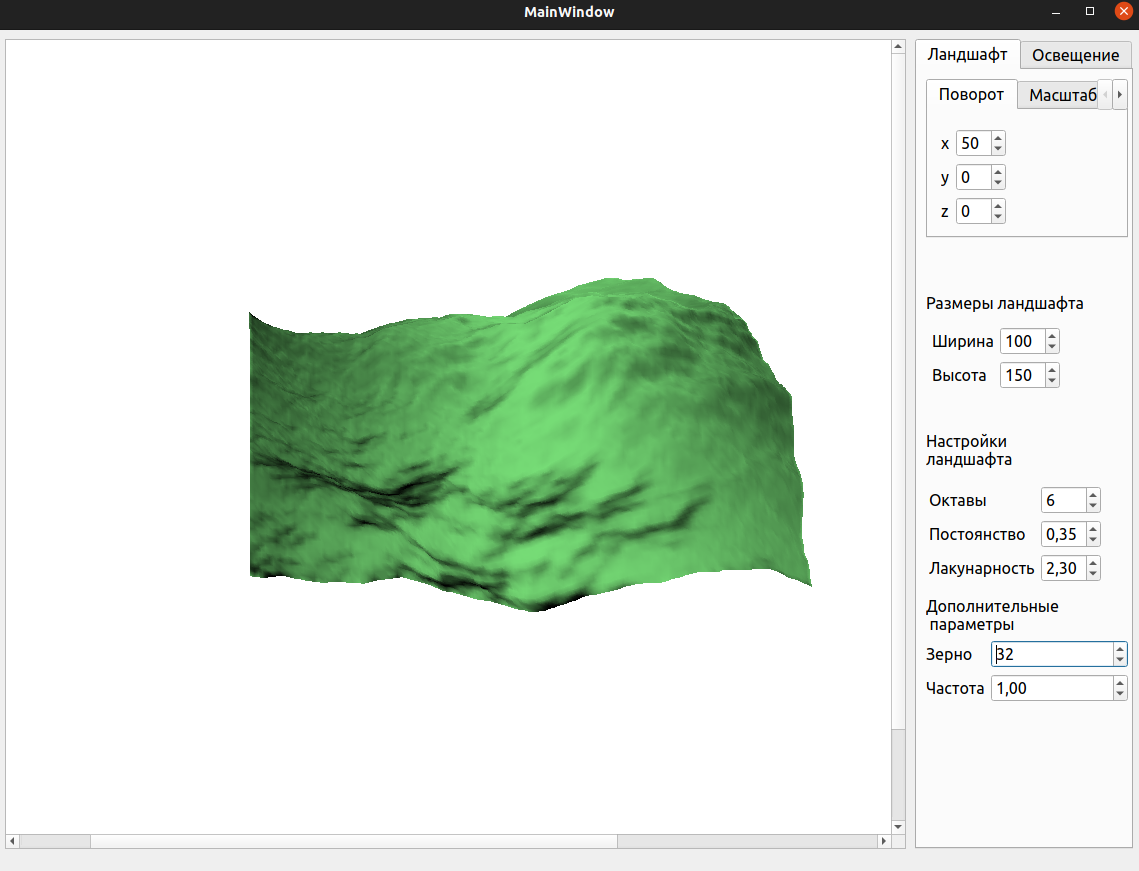
\includegraphics[scale=0.4]{../../../../../../../msys64/home/Лев/bmstu_cg_course_project/rpz/interface/interface_3}
		\caption{Интерфейс ПО}
		\label{png:interface_1}
	}
\end{figure}

Пользователь может изменять вид ландшафта следующим образом:
\begin{itemize}
	\item при помощи изменения параметров ландшафта (октавы, постоянство, лакунарность);
	\item для получения новой модели можно задать дополнительный параметр «Зерно»;
	\item изменять положение точечного источника света;
	\item осуществить поворот и масштабирование ландшафта.
\end{itemize}
	
Настройка параметров приведена на рисунках \ref{png:interface_params_1}, \ref{png:interface_params_2} и \ref{png:interface_params_3}.

\begin{figure}[H]
	\centering{
		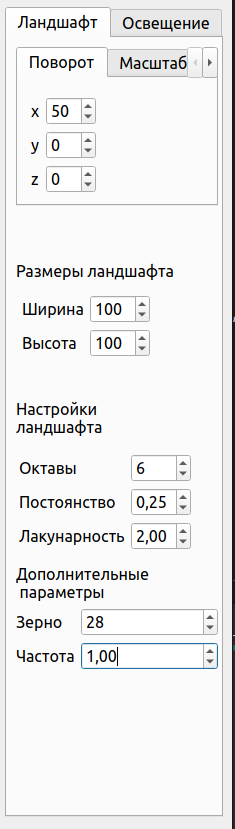
\includegraphics[scale=0.7]{../../../../../../../msys64/home/Лев/bmstu_cg_course_project/rpz/interface/interface_params_1}
		\caption{Изменение настроек ландшафта}
		\label{png:interface_params_1}
	}
\end{figure}

\begin{figure}[H]
	\centering{
		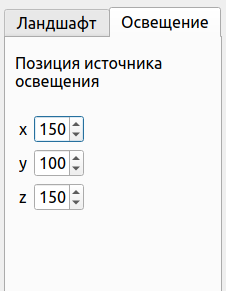
\includegraphics[scale=0.6]{../../../../../../../msys64/home/Лев/bmstu_cg_course_project/rpz/interface/interface_params_2}
		\caption{Изменение позиции источника освещения}
		\label{png:interface_params_2}
	}
\end{figure}

\begin{figure}[H]
	\centering{
		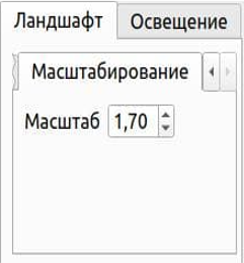
\includegraphics[scale=0.9]{../../../../../../../msys64/home/Лев/bmstu_cg_course_project/rpz/interface/interface_params_3}
		\caption{Изменение масштаба ландшафта}
		\label{png:interface_params_3}
	}
\end{figure}

	
\section{Вывод}
В данном разделе были выбраны средства реализации, среда разработки, приведены листинги модулей, представлен интерфейс ПО.